
\section{The \BaFePAs series}

The \BaFeAsP series progresses from \BaFeAs which becomes antiferromagnetic at around \unit[138]{K} and \BaFeP which is metallic to low temperatures. Neither end members are superconducting, however as arsenic is substituted for phosphor, the low temperature antiferromagnetic state decays, giving way to superconductivity which kicks in at approximately $x=0.18$ and increases to the optimal substitution of $x=0.31$ and then decreases until it gives way to a paramagnetic ground state at around $x=0.71$. \Fig\ref{Fig:3:PhaseDiagram} shows the phase diagram adapated ref. \cite{Nakai2010a} as determined by resistivety measurements.

\begin{figure}
    \begin{center}
        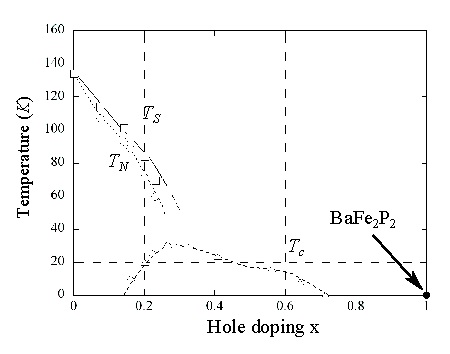
\includegraphics[scale=0.7]{Chapter3-dHvABaFe2P2/Figures/BaFe2P2Series/PhaseDiagram/PhaseDiagram}
        \caption{Phase diagram adapted from ref \cite{Nakai2010a} measured by resistivity. $T_s$, $T_N$ and $T_c$ are the structural transition, the antiferromagnetic transition and the superconducting transition temperatures respectively.}
        \label{Fig:3:PhaseDiagram}
    \end{center}
\end{figure}

 The progression along the series is isovalent as P and As are the same periodic group. The net effect of the substitution is to apply an increasing chemical pressure as $x$ moves towards $1$. Several reports show that applying \textit{physical} pressure to \BaFeAs results in a similar phase diagram with an antiferromagnetic phase and superconductivity up to $\sim$\unit[30]{K}\cite{Yamazaki2010,Colombier2009,Alireza2009} and in Klintberg \textit{et al.}\cite{Klintberg2010} a direct comparison has been made between the two. 
Structurally, the unit cell of the series is tetragonal ($I4/mmm$) for most of the phase diagram, aside from an orthorhombic phase below the $T_s$ line as shown in \fig\ref{Fig:3:PhaseDiagram}. The unit cell $a$ axis shrinks slightly less as pressure is applied compared with the $c$ axis ($\sim3\%$ c.f. $\sim4.5\%$ respectively). Interestingly though the $c$ axis shrinking largely occurs in the Fe-Pnictide plane leading to some theories of the superconductivity emerging from the tetrahedral bond angle between the Fe and the pnictigen.

\begin{figure}
    \begin{center}
        
\includegraphics[scale=0.7]{Chapter3-dHvABaFe2P2/Figures/BaFe2P2Series/UnitCell/UnitCell}
        \caption{The tetragonal unit cell of the 122 \BaFeAsP series.}
        \label{Fig:3:UnitCell}
    \end{center}
\end{figure}

By measuring the 

The \BaFePAs series has been previously measured by members of the group at Bristol using dHvA oscillations\cite{Shishido2010}. The electron surfaces have been characterised for x ranging from $0.41$ to $1$ and have clearly shown that the DFT calculations consistently overestimate the size of the surfaces. Moreover, dHvA measurements on the material with $x=0.63$ have been performed where one of the hole sheets was observed\cite{Analytis2010c}.
